\section{Metodologia}\label{sec:metodologia}

A metodologia consiste na formulação do dimensionamento de pontes de madeira roliça como um problema de otimização robusta multiobjetivo, totalmente acoplado a um modelo estrutural paramétrico e verificado segundo a ABNT NBR 7190 \parencite{NBR7190-1:2022}, com as ações determinadas conforme as ABNT NBR 6120 \parencite{NBR6120:2019} e ABNT NBR 7188 \parencite{nbr7188}. A plataforma computacional foi desenvolvida em linguagem \textit{Python}, adotando arquitetura cliente-servidor, com interface web construída com a biblioteca \textit{Streamlit} e disponível em acesso livre \parencite{ReliaBridge2026}.

O fluxo metodológico, ilustrado na Figura~\ref{fig:fluxograma}, é composto pelas seguintes etapas: (i) definição da geometria e das cargas permanentes; (ii) definição do trem tipo; (iii) cálculo estrutural dos esforços solicitantes e deslocamentos; (iv) combinação de ações nos estados limites último e de serviço; (v) determinação das resistências de projeto; (vi) verificações estruturais; (vii) otimização robusta via NSGA-II; e (viii) obtenção do conjunto de soluções viáveis da fronteira eficiente.

\begin{figure}[!ht]
    \centering
    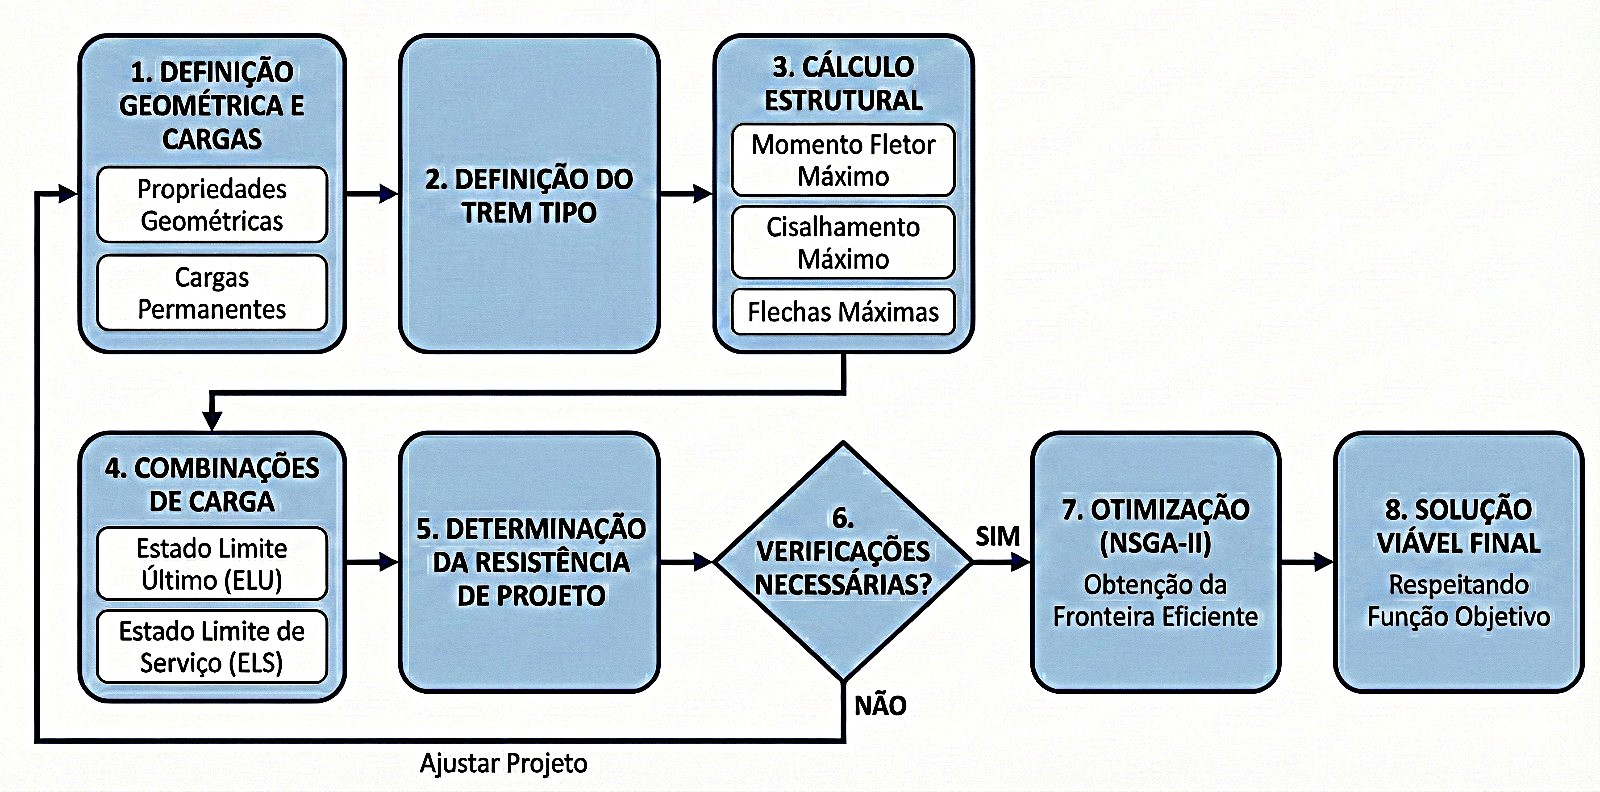
\includegraphics[width=0.9\textwidth]{figuras/fluxograma.jpeg}
    \caption{Fluxograma da otimização do dimensionamento de pontes de madeira.}
    \label{fig:fluxograma}
\end{figure}

\subsection{Sistema estrutural e modelo paramétrico}\label{sec:sistema}

O sistema estrutural considerado consiste em um tabuleiro de madeira composto por pranchas longitudinais retangulares, apoiadas sobre vigas longitudinais circulares de madeira roliça (longarinas), regularmente espaçadas a uma distância denominada espaçamento ($esp$). O tabuleiro está sujeito a ações permanentes (peso próprio) e a ações variáveis associadas ao tráfego (carga móvel). As cargas atuantes no tabuleiro são transferidas para as longarinas de apoio e modeladas como carregamentos uniformemente distribuídos ao longo do vão. A Figura~\ref{fig:sistema} apresenta a representação conceitual do sistema estrutural.

\begin{figure}[!ht]
    \centering
    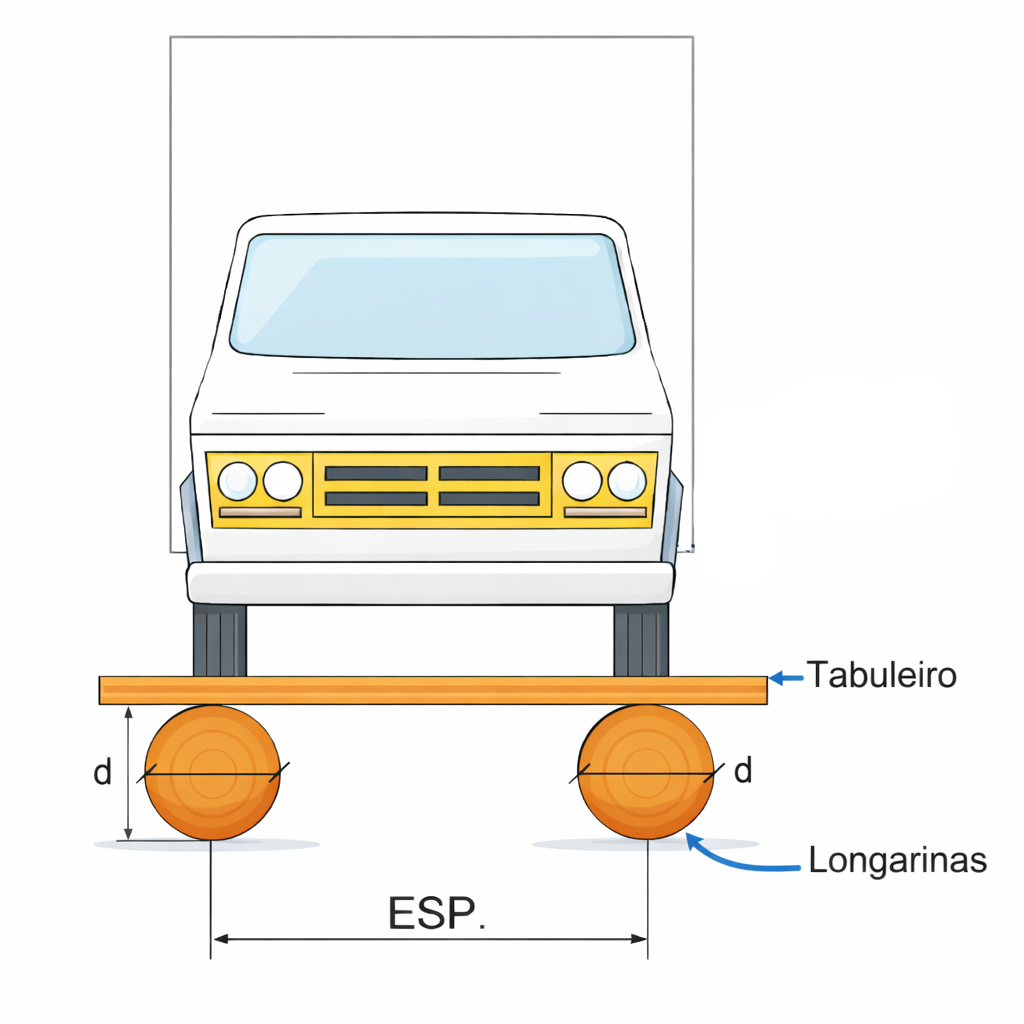
\includegraphics[width=0.5\textwidth]{figuras/caminhao.png}
    \caption{Representação conceitual do sistema estrutural da ponte de madeira.}
    \label{fig:sistema}
\end{figure}

O modelo é totalmente paramétrico: a partir de um conjunto de parâmetros de entrada (vão, largura da pista, propriedades mecânicas da madeira, classe de umidade, classe de carregamento, coeficientes normativos e trem tipo), as propriedades geométricas das seções e os esforços solicitantes são recalculados automaticamente para qualquer combinação das variáveis de projeto. Esse caráter paramétrico é o que possibilita o acoplamento direto com o algoritmo de otimização, uma vez que cada indivíduo avaliado corresponde a uma configuração geométrica completa da ponte.

\subsection{Formulação da otimização multiobjetivo}\label{sec:formulacao}

Um problema de otimização multiobjetivo envolve a minimização simultânea de múltiplas funções objetivo sujeitas a um conjunto de restrições, conforme a Equação~\eqref{eq:mop}.

\begin{equation}
\begin{cases}
\min\ f_m(\mathbf{x}), & m = 1,2,\ldots,M; \\
g_j(\mathbf{x}) \leq 0, & j = 1,2,\ldots,J; \\
h_k(\mathbf{x}) = 0, & k = 1,2,\ldots,K; \\
x_i^{(L)} \leq x_i \leq x_i^{(U)}, & i = 1,2,\ldots,n.
\end{cases}
\label{eq:mop}
\end{equation}

Diferentemente da otimização monoobjetivo, o problema não conduz a uma única solução ótima, mas a um conjunto de soluções ótimas de Pareto. Dadas duas soluções candidatas $\mathbf{x}^a$ e $\mathbf{x}^b$, diz-se que $\mathbf{x}^a$ domina $\mathbf{x}^b$ ($\mathbf{x}^a \prec \mathbf{x}^b$) se atende às condições da Equação~\eqref{eq:dominancia}.

\begin{equation}
\forall m \in \{1,\ldots,M\},\ f_m(\mathbf{x}^a) \leq f_m(\mathbf{x}^b)
\quad \text{e} \quad
\exists m\ :\ f_m(\mathbf{x}^a) < f_m(\mathbf{x}^b)
\label{eq:dominancia}
\end{equation}

O vetor de variáveis de projeto é $\mathbf{x} = (d, b_w, h, n_{long}, n_{tab})^T$, composto pelo diâmetro da longarina circular ($d$), pela largura ($b_w$) e altura ($h$) da seção transversal das pranchas do tabuleiro, e pelos parâmetros de espaçamento das longarinas ($n_{long}$) e das peças do tabuleiro ($n_{tab}$). As propriedades da seção da longarina dependem diretamente de seu diâmetro, o qual influencia a rigidez, a resistência e o peso próprio. O espaçamento e as dimensões do tabuleiro condicionam a distribuição de esforços e os níveis de deformação do conjunto.

O problema é formulado com duas funções objetivo antagônicas. A primeira consiste na minimização da área total de madeira, conforme a Equação~\eqref{eq:f1}.

\begin{equation}
f_1(\mathbf{x}) = A_{\mathrm{total}} = n_{long}\,A_{long}\,L + n_{tab}\,A_{tab}\,b_{w,\mathrm{pista}}
\label{eq:f1}
\end{equation}

A segunda função objetivo visa maximizar o desempenho estrutural em serviço, expresso pela relação entre o deslocamento total e o deslocamento limite. Para manter a estrutura de minimização, essa função é definida com sinal negativo, conforme a Equação~\eqref{eq:f2}.

\begin{equation}
f_2(\mathbf{x}) = -\,\frac{\delta_{\mathrm{tot}}}{\delta_{\mathrm{lim}}} = -\,\frac{\delta_{\mathrm{tot}}}{L/250}
\label{eq:f2}
\end{equation}

Onde $\delta_{\mathrm{tot}}$ é o deslocamento total no meio do vão da longarina sob a combinação das ações permanentes e variáveis, e $\delta_{\mathrm{lim}} = L/250$ é o limite admissível de deslocamento. Os objetivos são antagônicos, pois a redução da área tende a intensificar as deformações, enquanto o aumento da rigidez demanda maior quantidade de material.

O problema está sujeito às restrições estruturais associadas aos estados limites último e de serviço. Para a longarina, impõem-se a restrição de tensão normal à flexão (Equação~\eqref{eq:g1}), a restrição de tensão de cisalhamento (Equação~\eqref{eq:g2}) e a restrição de deslocamentos (Equação~\eqref{eq:g3}). Para o tabuleiro, impõe-se a restrição de tensão normal à flexão (Equação~\eqref{eq:g4}).

\begin{equation}
g_{1}(\mathbf{x}) = \frac{\sigma_{Sd}^{(l)}}{\sigma_{Rd}^{(l)}} - 1 \leq 0
\label{eq:g1}
\end{equation}

\begin{equation}
g_{2}(\mathbf{x}) = \frac{\tau_{Sd}^{(l)}}{\tau_{Rd}^{(l)}} - 1 \leq 0
\label{eq:g2}
\end{equation}

\begin{equation}
g_{3}(\mathbf{x}) = \max\left(\frac{\delta_{\mathrm{tot}}^{(l)}}{L/250},\ \frac{\delta_{qk}^{(l)}}{L/360}\right) - 1 \leq 0
\label{eq:g3}
\end{equation}

\begin{equation}
g_{4}(\mathbf{x}) = \frac{\sigma_{Sd}^{(t)}}{\sigma_{Rd}^{(t)}} - 1 \leq 0
\label{eq:g4}
\end{equation}

Adicionalmente, duas restrições geométricas ($g_5$ e $g_6$) garantem que o número inteiro de longarinas e de peças do tabuleiro preencha, de forma admissível, os espaços disponíveis da pista e do vão. O tratamento das restrições segue a abordagem baseada em viabilidade implementada na biblioteca \texttt{pymoo} \parencite{blank2020}: soluções viáveis sempre dominam soluções inviáveis; entre soluções viáveis aplica-se a dominância de Pareto; e entre soluções inviáveis a ordenação baseia-se no grau total de violação das restrições \parencite{DEB2009}.

\subsection{Algoritmo de otimização NSGA-II}\label{sec:nsga2}

O problema é resolvido pelo Algoritmo Genético de Ordenação Não Dominada II (NSGA-II), um algoritmo evolutivo desenvolvido para aproximar o conjunto ótimo de Pareto em problemas com objetivos conflitantes \parencite{DEB2009}. O NSGA-II preserva a natureza multiobjetivo do problema e busca um conjunto diverso de soluções não dominadas, sem recorrer à escalarização das funções objetivo.

A cada geração, a população é ordenada em frentes sucessivas não dominadas $\mathcal{F}_1, \mathcal{F}_2, \ldots$, sendo $\mathcal{F}_1$ a aproximação corrente da fronteira de Pareto. Para preservar a diversidade ao longo da fronteira, o algoritmo emprega a distância de aglomeração (\textit{crowding distance}), calculada conforme a Equação~\eqref{eq:crowding}.

\begin{equation}
d_i = \sum_{m=1}^{M} \frac{f_m(\mathbf{x}_{i+1}) - f_m(\mathbf{x}_{i-1})}{f_m^{\max} - f_m^{\min}}
\label{eq:crowding}
\end{equation}

Uma estratégia elitista combina as populações parental e descendente, selecionando os melhores indivíduos com base no nível de Pareto e na distância de aglomeração. O Algoritmo~\ref{alg:nsga2} resume a lógica de busca acoplada ao modelo estrutural e à avaliação robusta descrita na Seção~\ref{sec:robustez}.

\begin{algorithm}[!ht]
\caption{Otimização robusta multiobjetivo via NSGA-II acoplada ao modelo estrutural}\label{alg:nsga2}
\begin{algorithmic}[1]
\Require Limites $[x_i^{(L)}, x_i^{(U)}]$, tamanho da população $N_{pop}$, gerações $N_{gen}$, desvio de robustez $\rho$, número de checagens $N_c$
\Ensure Fronteira eficiente $\mathcal{F}_1$
\State Inicializar população $P_0$ por amostragem aleatória em $[x_i^{(L)}, x_i^{(U)}]$
\For{cada geração $t = 0$ até $N_{gen}-1$}
    \For{cada indivíduo $\mathbf{x} \in P_t$}
        \State $\mathbf{F} \gets \mathbf{0}$;\ $\mathbf{G} \gets \mathbf{0}$
        \For{$c = 1$ até $N_c$} \Comment{avaliação robusta}
            \State $\tilde{\mathbf{x}} \gets \mathbf{x}\,(1 + \rho\,\boldsymbol{\xi})$, com $\boldsymbol{\xi} \sim \mathcal{U}(-1,1)$
            \State $(\mathbf{f}, \mathbf{g}) \gets$ \Call{VerificaEstrutura}{$\tilde{\mathbf{x}}$} \Comment{NBR 7190}
            \State $\mathbf{F} \gets \mathbf{F} + \mathbf{f}$;\ $\mathbf{G} \gets \mathbf{G} + \mathbf{g}$
        \EndFor
        \State $\mathbf{F} \gets \mathbf{F}/N_c$;\ $\mathbf{G} \gets \mathbf{G}/N_c$ \Comment{agregação por média}
    \EndFor
    \State $Q_t \gets$ seleção por torneio, cruzamento SBX e mutação polinomial sobre $P_t$
    \State $R_t \gets P_t \cup Q_t$
    \State Ordenar $R_t$ em frentes não dominadas $\{\mathcal{F}_1, \mathcal{F}_2, \ldots\}$
    \State $P_{t+1} \gets$ melhores $N_{pop}$ indivíduos por nível de Pareto e distância de aglomeração
\EndFor
\State \Return $\mathcal{F}_1$
\end{algorithmic}
\end{algorithm}

Os parâmetros de configuração do NSGA-II adotados neste trabalho são apresentados na Tabela~\ref{tab:nsga2}. Foram empregados o operador de cruzamento SBX (\textit{Simulated Binary Crossover}) e o operador de mutação polinomial (PM), com eliminação de duplicatas, garantindo a diversidade da população ao longo das gerações.

\begin{table}[!ht]
\caption{Parâmetros de configuração do algoritmo NSGA-II.\label{tab:nsga2}}
\begin{threeparttable}
\begin{tabular*}{\columnwidth}{@{\extracolsep\fill}ll@{\extracolsep\fill}}
\toprule
Parâmetro & Valor \\
\midrule
Tamanho da população, $N_{pop}$ & 500 \\
Número de gerações, $N_{gen}$ & 400 \\
Cruzamento (SBX): probabilidade / $\eta$ & 0{,}90 / 15 \\
Mutação polinomial (PM): $\eta$ & 20 \\
Eliminação de duplicatas & Sim \\
Semente aleatória & 1 \\
\bottomrule
\end{tabular*}
\end{threeparttable}
\end{table}

\subsection{Avaliação da robustez}\label{sec:robustez}

A otimização determinística tende a posicionar as soluções ótimas exatamente sobre a fronteira das restrições ativas, tornando-as sensíveis a pequenas variações nas variáveis de projeto. Em pontes de madeira roliça, essa sensibilidade é agravada pela variabilidade natural do diâmetro das peças e pelas tolerâncias de fabricação e montagem. Para mitigar esse efeito, a robustez foi incorporada de forma nativa ao processo de busca.

A estratégia adotada consiste em avaliar cada solução candidata não apenas em seus valores nominais, mas sob um conjunto de perturbações aplicadas às variáveis de projeto. Para um indivíduo $\mathbf{x}$, geram-se $N_c$ realizações perturbadas $\tilde{\mathbf{x}}^{(c)}$ conforme a Equação~\eqref{eq:perturbacao}.

\begin{equation}
\tilde{x}_i^{(c)} = x_i \left(1 + \rho\,\xi_i^{(c)}\right),
\qquad \xi_i^{(c)} \sim \mathcal{U}(-1,\,1),
\qquad \rho = 0{,}05
\label{eq:perturbacao}
\end{equation}

Onde $\rho = 0{,}05$ corresponde ao desvio de 5\% aplicado a todas as variáveis de projeto em relação aos seus valores nominais, e $\xi_i^{(c)}$ é uma variável aleatória uniforme no intervalo $[-1, 1]$. Cada uma das $N_c$ realizações é submetida à verificação estrutural completa segundo a ABNT NBR 7190 \parencite{NBR7190-1:2022}, e as funções objetivo e restrições são agregadas pela média, conforme as Equações~\eqref{eq:fmed} e~\eqref{eq:gmed}.

\begin{equation}
\bar{f}_m(\mathbf{x}) = \frac{1}{N_c}\sum_{c=1}^{N_c} f_m\!\left(\tilde{\mathbf{x}}^{(c)}\right)
\label{eq:fmed}
\end{equation}

\begin{equation}
\bar{g}_j(\mathbf{x}) = \frac{1}{N_c}\sum_{c=1}^{N_c} g_j\!\left(\tilde{\mathbf{x}}^{(c)}\right)
\label{eq:gmed}
\end{equation}

Dessa forma, uma solução só é considerada viável e economicamente vantajosa se mantiver o atendimento às restrições, em média, mesmo quando suas variáveis de projeto oscilam dentro da faixa de $\pm 5\%$. Soluções posicionadas exatamente sobre o limite de uma restrição passam a apresentar violação em parte das realizações perturbadas, elevando o valor médio $\bar{g}_j$ e sendo, portanto, penalizadas pelo mecanismo de viabilidade do NSGA-II. O efeito prático é o deslocamento da fronteira eficiente para o interior do domínio viável, resultando em soluções com margem de segurança adicional em troca de um acréscimo controlado no consumo de material. O número de checagens $N_c$ controla a estabilidade da estimativa do valor médio: valores maiores reduzem a variância da avaliação, ao custo de maior esforço computacional.

\sugestao{Inserir estudo de sensibilidade do parâmetro de robustez, plotando a fronteira eficiente para $\rho = 0\%$, $2{,}5\%$, $5\%$ e $10\%$, quantificando o acréscimo percentual de área (custo da robustez) em função do nível de desvio adotado. Este gráfico evidencia o \textit{trade-off} entre economia de material e tolerância a incertezas, resultado de forte apelo para periódicos de alto impacto.}

\sugestao{Comparar a estratégia de agregação pela média com uma formulação de pior caso (min-max robusto), $\bar{g}_j = \max_c g_j(\tilde{\mathbf{x}}^{(c)})$, e discutir o impacto de cada abordagem sobre a probabilidade de falha das soluções da fronteira, conectando a otimização robusta a uma análise de confiabilidade estrutural via FORM ou Monte Carlo.}

\subsection{Dimensionamento estrutural segundo a NBR 7190}\label{sec:dimensionamento}

Esta seção apresenta os itens normativos e o equacionamento empregados na verificação dos elementos de madeira, os quais constituem a rotina \textsc{VerificaEstrutura} invocada pelo Algoritmo~\ref{alg:nsga2}. As verificações abrangem os estados limites últimos associados às tensões normais e tangenciais e o estado limite de serviço relacionado a deslocamentos.

\subsubsection{Propriedades geométricas da seção transversal}

Para a longarina circular maciça de diâmetro $d$, a área, o momento de inércia, o módulo resistente e o raio de giração são obtidos pelas Equações~\eqref{eq:areacirc} a~\eqref{eq:rcirc}.

\begin{equation}
A = \frac{\pi d^2}{4}
\label{eq:areacirc}
\end{equation}

\begin{equation}
I_x = I_y = \frac{\pi d^4}{64}
\label{eq:icirc}
\end{equation}

\begin{equation}
W_x = W_y = \frac{I_x}{d/2}
\label{eq:wcirc}
\end{equation}

\begin{equation}
r_x = r_y = \sqrt{\frac{I_x}{A}}
\label{eq:rcirc}
\end{equation}

Para as pranchas retangulares do tabuleiro, de largura $b_w$ e altura $h$, a área e o momento de inércia em relação ao eixo de flexão são dados pelas Equações~\eqref{eq:arearet} e~\eqref{eq:iret}.

\begin{equation}
A = b_w\,h
\label{eq:arearet}
\end{equation}

\begin{equation}
I_x = \frac{b_w\,h^3}{12}
\label{eq:iret}
\end{equation}

\subsubsection{Ações permanentes e trem tipo}

As ações permanentes correspondem ao peso próprio das longarinas, do tabuleiro e demais elementos, obtidas em função da geometria e do peso específico, conforme a Equação~\eqref{eq:permanente}.

\begin{equation}
G = \gamma \cdot A
\label{eq:permanente}
\end{equation}

A carga móvel rodoviária é definida pela ABNT NBR 7188 \parencite{nbr7188}. Para estradas vicinais, a norma admite o trem tipo mínimo TB-240, representado por um veículo de 240~kN com três eixos e seis rodas, cada roda transmitindo 40~kN, espaçamento de 1{,}5~m entre eixos, e carga de multidão de 4{,}0~kN/m\textsuperscript{2}. O trem tipo TB-450 corresponde a um veículo de 450~kN, com roda de 75~kN e carga de multidão de 5{,}0~kN/m\textsuperscript{2}. A Figura~\ref{fig:trem} ilustra a configuração do trem tipo.

\begin{figure}[!ht]
    \centering
    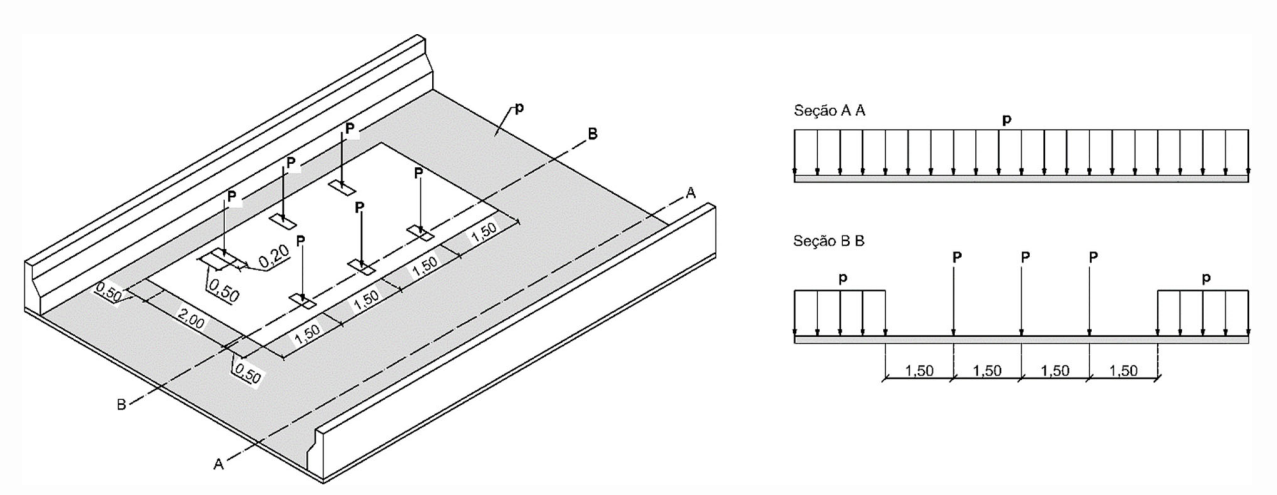
\includegraphics[width=0.95\textwidth]{figuras/trem_tipo.png}
    \caption{Configuração do trem tipo rodoviário.}
    \label{fig:trem}
\end{figure}

Os efeitos dinâmicos são incorporados pelo coeficiente de impacto vertical ($CIV$), determinado pelas Equações~\eqref{eq:civ1} e~\eqref{eq:civ2}, em que $LIV$ é o comprimento característico da estrutura.

\begin{equation}
CIV = 1{,}35, \qquad \text{para } L \leq 10{,}0\ \text{m}
\label{eq:civ1}
\end{equation}

\begin{equation}
CIV = 1 + 1{,}06\left(\frac{20}{LIV + 50}\right), \qquad \text{para } 10{,}0 < L \leq 200{,}0\ \text{m}
\label{eq:civ2}
\end{equation}

\subsubsection{Esforços solicitantes}

O momento fletor máximo devido à carga permanente, para viga biapoiada sob carga uniformemente distribuída, é dado pela Equação~\eqref{eq:mgk} \parencite{CALIL2006}. Para a carga variável das classes 30 e 45, o momento depende da extensão do vão, conforme as Equações~\eqref{eq:mqk30} e~\eqref{eq:mqk45}.

\begin{equation}
M_{gk} = \frac{q\,L^2}{8}
\label{eq:mgk}
\end{equation}

\begin{equation}
M_{qk} = \frac{3\,P\,L}{4} - P\,a, \qquad \text{para } 3\,\text{m} < L \leq 6\,\text{m}
\label{eq:mqk30}
\end{equation}

\begin{equation}
M_{qk} = \left(\frac{3\,P\,L}{4} - P\,a\right) + \frac{q\,c^2}{2}, \qquad \text{para } L > 6\,\text{m}
\label{eq:mqk45}
\end{equation}

O esforço cortante máximo devido à carga permanente é dado pela Equação~\eqref{eq:qgk}, e a parcela reduzida da carga variável pela Equação~\eqref{eq:qqk}, em que $e = L - 3a - 2h$.

\begin{equation}
Q_{gk} = \frac{g\,L}{2}
\label{eq:qgk}
\end{equation}

\begin{equation}
Q_{qk} = \frac{P}{L}\,(6a + 3e) + \frac{q\,e^2}{2\,L}
\label{eq:qqk}
\end{equation}

A flecha máxima devida à carga permanente é dada pela Equação~\eqref{eq:flechag} e a parcela devida à carga concentrada de roda pela Equação~\eqref{eq:flechaq}, com $b = (L-2a)/2$.

\begin{equation}
\delta_{gk} = \frac{5\,g\,L^4}{384\,E_{0,\mathrm{ef}}\,I}
\label{eq:flechag}
\end{equation}

\begin{equation}
\delta_{qk} = \frac{P}{48\,E_{0,\mathrm{ef}}\,I}\left[L^3 + 2\,b\left(3L^2 - 4b^2\right)\right]
\label{eq:flechaq}
\end{equation}

\subsubsection{Combinações e resistências de projeto}

No estado limite último adota-se a combinação última normal da ABNT NBR 8681 \parencite{NBR8681:2025}, conforme a Equação~\eqref{eq:comb}. As resistências de cálculo são obtidas pela Equação~\eqref{eq:xd}, com o coeficiente de modificação dado pelo produto $k_{mod} = k_{mod,1}\,k_{mod,2}$, e coeficientes de minoração $\gamma_{wf} = 1{,}4$ (tensões normais) e $\gamma_{wc} = 1{,}8$ (cisalhamento).

\begin{equation}
F_d = \sum_{i=1}^{m}\gamma_{gi}\,F_{Gi,k} + \gamma_{q1}\,F_{Q1,k} + \sum_{j=2}^{n}\gamma_{qj}\,\psi_{0j}\,F_{Qj,k}
\label{eq:comb}
\end{equation}

\begin{equation}
X_d = k_{mod}\,\frac{X_k}{\gamma_m}
\label{eq:xd}
\end{equation}

\subsubsection{Verificações de segurança}

A verificação à flexão compara a tensão normal solicitante com a resistência de cálculo (Equação~\eqref{eq:verflexao}). A verificação ao cisalhamento, para a seção circular, emprega a tensão máxima no centro da seção (Equação~\eqref{eq:vercis}) \parencite{Moraes2023}. A verificação de serviço compara a flecha total com o limite admissível.

\begin{equation}
\frac{\sigma_{Mx,d}}{f_{m,d}} = \frac{M_d}{W\,f_{m,d}} \leq 1
\label{eq:verflexao}
\end{equation}

\begin{equation}
\tau_{\max} = \frac{4}{3}\cdot\frac{Q_d}{A} \leq f_{v0,d}
\label{eq:vercis}
\end{equation}

Para cada verificação define-se uma função limite $g = (\text{solicitante}/\text{resistente}) - 1$, sendo o elemento considerado seguro quando $g < 0$. Essas funções limite são exatamente as restrições $g_1$ a $g_4$ da formulação de otimização (Equações~\eqref{eq:g1} a~\eqref{eq:g4}), o que garante o acoplamento integral entre o dimensionamento normativo e o processo de busca.

\subsection{Demonstração do dimensionamento}\label{sec:demonstracao}

Para ilustrar a rotina de verificação empregada em cada avaliação do NSGA-II, apresenta-se o dimensionamento completo de uma longarina circular submetida ao trem tipo TB-240, adotando $d = 0{,}60$~m, $L = 5{,}0$~m, $esp = 1{,}20$~m, madeira com $f_{mk} = 50$~MPa, $f_{vk} = 4{,}0$~MPa, $E_{0,\mathrm{ef}} = 14$~GPa e densidade de 620~kg/m\textsuperscript{3}.

As propriedades geométricas resultam em $A = 0{,}2827$~m\textsuperscript{2}, $I_x = 0{,}0064$~m\textsuperscript{4} e $W_x = 0{,}0212$~m\textsuperscript{3}. Com $k_{mod} = 0{,}60 \times 1{,}00 = 0{,}60$, as resistências de cálculo são $f_{md} = 0{,}60 \times 50/1{,}40 = 21{,}43$~MPa e $f_{vd} = 0{,}60 \times 4{,}0/1{,}80 = 1{,}33$~MPa.

A carga permanente total na longarina, somando o peso próprio do tabuleiro, a carga permanente aplicada e o peso próprio da longarina, resulta em $Q_{lon} = 5{,}108$~kN/m, conduzindo a $M_{gk} = 5{,}108 \times 5{,}0^2/8 = 15{,}96$~kN$\cdot$m. O momento devido às rodas é $M_{qk} = (3\times40\times5{,}0)/4 - 40\times1{,}5 = 90{,}00$~kN$\cdot$m, corrigido pelo impacto vertical ($CIV = 1{,}35$) para $M_{qk,\mathrm{corr}} = 113{,}63$~kN$\cdot$m. A combinação última fornece $M_{sd} = 1{,}35\times15{,}96 + 1{,}50\times113{,}63 = 191{,}99$~kN$\cdot$m, resultando em $\sigma_x = 191{,}99/0{,}0212 = 9\,053{,}5$~kPa e função limite $g = 9\,053{,}5/21\,428{,}6 - 1 = -0{,}57 < 0$ (seguro).

De forma análoga, a verificação ao cisalhamento conduz a $V_{sd} = 122{,}15$~kN, $\tau_{sd} = (4/3)\times122{,}15/0{,}2827 = 576{,}0$~kPa e $g = 576{,}0/1\,333{,}3 - 1 = -0{,}57 < 0$ (seguro). A verificação de serviço fornece flecha total $\delta_{sd} = 0{,}00167$~m frente ao limite $\delta_{lim} = L/250 = 0{,}020$~m, com $g = -0{,}916 < 0$ (seguro). O tabuleiro, verificado para vão de influência de 1{,}20~m, apresenta $\sigma_x = 9{,}51$~MPa frente a $f_{md} = 21{,}43$~MPa, com $g = -0{,}556 < 0$ (seguro). Esse conjunto de funções limite é o que alimenta o vetor de restrições avaliado, sob perturbação de 5\%, a cada geração do algoritmo.
